

\section{Network Requirements and Structure}

A network both defines the composition advected by the hydro code as
well as describes the burning processes between those isotopes.
Evolving the species in a network requires an integrator.  The design
of \microphysics\ decouples the integrator from the network, allowing
for the ability to swap integrators as desired.  We discuss the
integrators in a later section.


At a minimum, a network needs to provide:
\begin{itemize}
 \item {\tt nspec} : the number of species in the network

 \item {\tt nspec\_evolve} : the number of species that are actually
   integrated in the network.  Usually this is {\tt nspec}, but in general
   any {\tt nspec\_evolve} $\le$ {\tt nspec} is allowed.  Those species
   not evolved are held constant in the integration.

   Note that the convention is that the first {\tt nspec\_evolve} out
   of the {\tt nspec} species are the ones evolved.

 \item {\tt nrates} : the number of reaction rates.  This is used to
   cache rates for the analytic Jacobian.

 \item {\tt naux} : the number of auxiliary quantities needed by the
   network (these are not evolved).  \MarginPar{does any net use these?}

 \item {\tt aion(:)} : the atomic weight (in atomic mass units) of the
   species

 \item {\tt zion(:)} : the atomic number of the species

 \item {\tt spec\_names(:)} : a descriptive name of the species
   (e.g. {\tt "hydrogen-1"})

 \item {\tt short\_spec\_names(:)} : a shorten version of the species name
   (e.g. {\tt "H1"})

 \item {\tt short\_aux\_names(:)} : the names of the auxiliary quantities

 \item {\tt network\_name} : a descriptive name for the network

\end{itemize}
Most of these quantities are Fortran parameters.

{\bf A convention adopted in \microphysics\ is that each network
is responsible for determining the energy release from a change
in composition}.  Most networks will provide an array of the species
binding energies and a routine to compute the energy yield from
the reaction rates.

There are three primary files within each network directory.

\begin{itemize}

\item {\tt actual\_network.f90}:

  This is the Fortran module {\tt actual\_network} with routines:
  \begin{itemize}
  \item {\tt actual\_network\_init()}
  \item {\tt actual\_network\_finalize()}
  \end{itemize}

  This supplies the number and names of species and auxiliary
  variables, as well as other initializing data, such as their mass
  numbers, proton numbers, and binding energies. It needs to define
  the {\tt nspec} and {\tt naux} quantities as integer
  parameters. Additionally it must define {\tt nspec\_evolve}, the
  number of species that are actually evolved during a burn; in most
  cases, this should have the same value as {\tt nspec}.  Finally, it
  must also define {\tt nrates}, the number of reaction rates linking
  the isotopes in the network.

\item {\tt actual\_rhs.f90}:

  This is the Fortran module {\tt actual\_rhs\_module}, with routines:
  \begin{itemize}
  \item {\tt actual\_rhs\_init()}
  \item {\tt actual\_rhs(state)}
  \item {\tt actual\_jac(state)}
  \end{itemize}

  This supplies an interface for computing the right-hand-side of the
  network, the time-derivative of each species (and the temperature
  and nuclear energy release), as well as the analytic Jacobian.
  Both {\tt actual\_rhs} and {\tt actual\_jac} take a single argument,
  a {\tt burn\_t} state.  They set the time-derivates and Jacobian
  elements in this derived type directly.

  Note: some networks do not provide an analytic Jacobian and instead
  rely on the numerical difference-approximation to the Jacobian.  In
  this case, the interface {\tt actual\_jac} is still needed to compile.

\item {\tt actual\_burner}:

  This is the Fortran module {\tt actual\_burner\_module}, with routines:
  \begin{itemize}
  \item {\tt actual\_burner\_init()}
  \item {\tt actual\_burner(state\_in, state\_out, dt, time)}
  \end{itemize}

  This contains the interface for doing an actual burn.  Here, {\tt
    state\_in} and {\tt state\_out} are {\tt burn\_t} objects.  In
  general, you will want to {\tt call integrator} to use one of the
  pre-defined ODE integrators, but you could also write a custom
  integration here. This is covered in more detail in \S~\ref{ch:networks:integrators}.

\end{itemize}

Notice that all three of these modules have initialization routines:
\begin{itemize}
  \item {\tt actual\_network\_init()}
  \item {\tt actual\_rhs\_init()}
  \item {\tt actual\_burner\_init()}
\end{itemize}
These must be called upon initialization. These should be not called
within OpenMP parallel regions, because in general they will modify
shared module data.

Note, depending on the network, some of these may do nothing, but
these interfaces are all required for maximum flexibility.


\section{Available Networks}


\subsection{{\tt aprox13}, {\tt aprox19}, and {\tt aprox21}}

These are alpha-chains (with some other nuclei) from Frank Timmes.
These networks share common rates (from {\tt Microphysics/rates}),
plasma neutrino loses (from {\tt Microphysics/neutrinos}), and
electron screening (from {\tt Microphysics/screening}).

\paragraph{Energy generation.} These networks store the total binding
energy of the nucleus in MeV as {\tt bion(:)}.  They then compute the
mass of each nucleus in grams as:
\begin{equation}
M_k = (A_k - Z_k) m_n + Z_k (m_p + m_e) - B_k
\end{equation}
where $m_n$, $m_p$, and $m_e$ are the neutron, proton, and electron
masses, $A_k$ and $Z_k$ are the atomic weight and number, and $B_k$
is the binding energy of the nucleus (converted to grams).  $M_k$
is stored as {\tt mion(:)} in the network.

The energy release per gram is converted from the rates as:
\begin{equation}
\edot = -N_A c^2 \sum_k \frac{dY_k}{dt} M_k - \edot_\nu
\end{equation}
where $N_A$ is Avogadro's number (to convert this to ``per gram'')
and $\edot_\nu$ is the neutrino loss term.

\subsection{{\tt breakout}}

\subsection{{\tt CONe2NSE}}

\subsection{{\tt general\_null}}

{\tt general\_null} is a bare interface for a nuclear reaction
network; no reactions are enabled, and no auxiliary variables are
accepted.  The data in the Fortran module is defined at compile type
by specifying an inputs file.  For example, {\tt
  Networks/general\_null/triple\_alpha\_plus\_o.net} would describe
the triple-$\alpha$ reaction converting helium into carbon, as well as
oxygen and iron.

At compile time, the network module {\tt actual\_network.f90}
is written using the python script {\tt write\_network.py}
and the template {\tt network.template}.  The {\tt make} rule
for this is contained in {\tt Make.package} (for \cpp\ \boxlib) and
{\tt GPackage.mak} (for F90 \boxlib).  The name of the inputs file
is specified by the variable {\tt GENERAL\_NET\_INPUTS}.

A version of this network comes with \maestro\ and \castro, so you do
not usually need to worry about the version in \microphysics.


\subsection{{\tt ignition\_chamulak}}

This network was introduced in our paper on convection in white dwarfs
as a model of Type Ia supernovae~\cite{wdconvect}.  It models
carbon burning in a regime appropriate for a simmering white dwarf,
and captures the effects of a much larger network by setting the ash
state and energetics to the values suggested in \cite{chamulak:2008}.

This network has {\tt nspec = 3}, but {\tt nspec\_evolve = 1}.  Only a
single reaction is modeled, converting \isot{C}{12} into ``{\tt
  ash}''.

\paragraph{Energy generation.} The binding energy, $q$, in this
network is interpolated based on the density.  It is stored as the
binding energy (ergs/g) {\em per nucleon}, with a sign convention that
binding energies are negative.  The energy generation rate is then:
\begin{equation}
\edot = q \frac{dX(\isotm{C}{12})}{dt} = q A_{\isotm{C}{12}} \frac{dY(\isotm{C}{12})}{dt}
\end{equation}
(this is positive since both $q$ and $dY/dt$ are negative)

\subsection{{\tt ignition\_reaclib}}

\subsection{{\tt ignition\_simple}}

This is the original network used in our white dwarf convection
studies~\cite{lowMach4}.  It includes a single-step
$^{12}\mathrm{C}(^{12}\mathrm{C},\gamma)^{24}\mathrm{Mg}$ reaction.
The carbon mass fraction equation appears as
\begin{equation}
\frac{D X(^{12}\mathrm{C})}{Dt} = - \frac{1}{12} \rho X(^{12}\mathrm{C})^2
    f_\mathrm{Coul} \left [N_A \left <\sigma v \right > \right]\enskip,
\end{equation}
where $N_A \left <\sigma v\right>$ is evaluated using the reaction
rate from (Caughlan and Fowler 1988).  The Coulomb screening factor,
$f_\mathrm{Coul}$, is evaluated using the general routine from the
Kepler stellar evolution code (Weaver 1978), which implements the work
of (Graboske 1973) for weak screening and the work of (Alastuey 1978
and Itoh 1979) for strong screening.


\subsection{{\tt iso7}}


\subsection{{\tt kpp}}


\subsection{{\tt powerlaw}}

This is a simple single-step reaction rate.
We will consider only two species, fuel, $f$, and ash, $a$, through
the reaction: $f + f \rightarrow a + \gamma$.  Baryon conservation
requres that $A_f = A_a/2$, and charge conservation requires that $Z_f
= Z_a/2$.  We take
our reaction rate to be a powerlaw in temperature.  The standard way
to write this is in terms of the number densities, in which case we
have
\begin{equation}
\frac{d n_f}{d t} = -2\frac{d n_a}{d t} = -r
\end{equation}
with
\begin{equation}
  r = r_0 n_X^2 \left( \frac{T}{T_0} \right )^\nu
\end{equation}
Here, $r_0$ sets the overall rate, with units of
$[\mathrm{cm^3~s^{-1}}]$, $T_0$ is a reference temperature scale, and
$\nu$ is the temperature exponent, which will play a role in setting
the reaction zone thickness.  In terms of mass fractions, $n_f = \rho
X_a / (A_a m_u)$, our rate equation is
\begin{eqnarray}
 \frac{dX_f}{dt} &=& - \frac{r_0}{m_u} \rho X_f^2 \frac{1}{A_f} \left (\frac{T}{T_0}\right)^\nu \equiv \omegadot_f \label{eq:Xf} \\
 \frac{dX_a}{dt} &=& \frac{1}{2}\frac{r_0}{m_u} \rho X_f^2 \frac{A_a}{A_f^2} \left (\frac{T}{T_0}\right)^\nu = \frac{r_0}{m_u} \rho X_f^2 \frac{1}{A_f} \left (\frac{T}{T_0}\right)^\nu  \label{eq:Xa}
\end{eqnarray}
We define a new rate constant, $\rt$ with units of $[\mathrm{s^{-1}}]$ as
\begin{equation}
\rt =  \begin{cases}
  \dfrac{r_0}{m_u A_f} \rho_0 & \text{if $T \ge T_a$} \\[1em]
  0                          & \text{if $T < T_a$}
 \end{cases}
\end{equation}
where $\rho_0$ is a reference density and $T_a$ is an activation
temperature, and then our mass fraction equation is:
\begin{equation}
\frac{dX_f}{dt} = -\rt X_f^2 \left (\frac{\rho}{\rho_0} \right ) \left ( \frac{T}{T_0}\right )^\nu
\end{equation}
Finally, for the
energy generation, we take our reaction to release a specific energy,
$[\mathrm{erg~g^{-1}}]$, of $\qburn$, and our energy source is
\begin{equation}
\epsdot = -\qburn \frac{dX_f}{dt}
\end{equation}

There are a number of parameters we use to control the constants in
this network.  This is one of the few networks that was designed
to work with {\tt gamma\_law\_general} as the EOS.

\subsection{{\tt rprox}}

This network contains 10 species, approximating hot CNO,
triple-$\alpha$, and rp-breakout burning up through \isot{Ni}{56},
using the ideas from \cite{wallacewoosley:1981}, but with modern
reaction rates from {\sf ReacLib}~\cite{ReacLib} where available.
This network was used for the X-ray burst studies in
\cite{xrb:II,xrb:III}, and more details are contained in those papers.


\subsection{{\tt triple\_alpha\_plus\_cago}}

This is a 2 reaction network for helium burning, capturing the $3$-$\alpha$
reaction and $\isotm{C}{12}(\alpha,\gamma)\isotm{O}{16}$.  Additionally,
\isot{Fe}{56} is included as an inert species.

This network has {\tt nspec = 4}, but {\tt nspec\_evolve = 3}.



\subsection{{\tt xrb\_simple}}

This is a simple 7 isotope network approximating the burning that
takes place in X-ray bursts (6 isotopes participate in reactions, one
additional, \isot{Fe}{56}, serves as an inert composition).  The 6 reactions
modeled are:
\begin{itemize}
\item $3\alpha + 2p \rightarrow \isotm{O}{14}$  (limited by the 3-$\alpha$ rate)

\item $\isotm{0}{14} + \alpha \rightarrow \isotm{Ne}{18}$
  (limited by $\isotm{O}{14}(\alpha,p)\isotm{F}{17}$ rate)

\item $\isotm{O}{15} + \alpha + 6 p \rightarrow \isotm{Si}{25}$
  (limited by $\isotm{O}{15}(\alpha,\gamma)\isotm{Ne}{19}$ rate)

\item $\isotm{Ne}{18} + \alpha + 3p \rightarrow \isotm{Si}{25}$
  (limited by $\isotm{Ne}{18}(\alpha,p)\isotm{Na}{21}$ rate)

\item $\isotm{O}{14} + p \rightarrow \isotm{O}{15}$
  (limited by $\isotm{O}{14}(e+\nu)\isotm{N}{14}$ rate)

\item $\isotm{O}{15} + 3p \rightarrow \isotm{O}{14} + \alpha$
  (limited by $\isotm{O}{15}(e+\nu)\isotm{N}{15}$ rate)
\end{itemize}
All reactions conserve mass.  Where charge is not conserved, fast weak
interactions are assumed.  Weak rates are trivial, fits to the 4
strong rates to a power law in $T_9 \in [0.3, 1]$, linear in density.



\section{Reaction ODE System}

The equations we integrate to do a nuclear burn are:
\begin{eqnarray}
  \frac{dY_k}{dt} &=& \omegadot_k(\rho,Y_k,T), \label{eq:spec_integrate} \\
  \frac{de}{dt} &=& f(\dot{Y}_k) \label{eq:enuc_integrate} \\
  \frac{dT}{dt} &=&\frac{\dot{e}}{c_x}. \label{eq:temp_integrate}
\end{eqnarray}
Here $Y_k \equiv X_k / A_k$ is the molar fraction of species $k$, where
$X_k$ is the mass fraction and $A_k$ is the mass number of that species.
$e$ is the internal energy, $T$ is the temperature\footnote{Note that in
previous versions of our networks in \castro\ and \maestro,
there was another term in the temperature equation relating to the
chemical potential of the gas as it came from the EOS. We have since
decided that this term should analytically cancel to zero in all cases
for our nuclear networks, and so we no longer think it is correct to
include a numerical approximation of it in the integration scheme. So
the current results given by our networks will in general be a little
different than in the past.}
, and $c_x$ is the specific heat for the fluid. The function $f$ provides
the energy release based on the instantaneous reaction terms, $\dot{Y}_k$.
As noted in the previous section, this is implemented in a network-specific
manner.

In this system, $e$ is not necessarily the total specific internal energy,
but rather just captures the energy release during the burn.

{\bf Note that while $Y_k$ is the integration variable, this is invisible to
the code that calls the burner---it hands the burner the mass fractions $X_k$
and gets back updated mass fractions.}


While this is the most common way to construct the set of
burn equations, and is used in most of our production networks,
all of them are ultimately implemented by the network itself, which
can choose to disable the evolution of any of these equations by
setting the RHS to zero. The integration software provides some
helper routines that construct common RHS evaluations, like the RHS
of the temperature equation given $\dot{e}$, but these calls
are always explicitly done by the individual networks rather than
being handled by the integration backend. This allows you to write a
new network that defines the RHS in whatever way you like.


\subsection{Interfaces}

The righthand side of the network is implemented by {\tt
  actual\_rhs()} in {\tt actual\_rhs.f90}, and appears as:
\begin{lstlisting}[language={[95]fortran}]
  subroutine actual_rhs(state)
    type (burn_t) :: state
\end{lstlisting}

All of the necessary integration data comes in through {\tt state}, as:
\begin{itemize}
\item {\tt state \% xn(:)} : the {\tt nspec} mass fractions (note: for
  the case that {\tt nspec\_evolve < nspec}, an algebraic constraint
  may need to be enforced.  See \S~\ref{ch:networks:nspec_evolve}).

\item {\tt state \% e} : the current value of the ODE system's energy 
  release---note: as discussed above, this is not necessarily the energy
  you would get by calling the EOS on the state.  It is very rare (never?)
  that a RHS implementation would need to use this variable.

\item {\tt state \% T} : the current temperature

\item {\tt state \% rho} : the current density
\end{itemize}
Note that we come in with the mass fractions, but the molar fractions can
be computed as:
\begin{lstlisting}[language={[95]fortran}]
  double precision :: y(nspec)
  ...
  y(:) = state % xn(:) / aion(:)
\end{lstlisting}

The {\tt actual\_rhs()} routine's job is to fill the righthand side vector
for the ODE system, {\tt state \% ydot(:)}.  Here, the important
fields to fill are:
\begin{itemize}
\item {\tt state \% ydot(1:nspec\_evolve)} : the change in {\em molar
  fractions} for the {\tt nspec\_evolve} species that we are evolving,
  $d({Y}_k)/dt$

\item {\tt state \% ydot(net\_ienuc)} : the change in the energy release 
  from the net, $de/dt$

\item {\tt state \% ydot(net\_itemp)} : the change in temperature, $dT/dt$
\end{itemize}

If the network builds the RHS in terms of mass fractions, $dX_k/dt$, then 
these will need to be converted to molar fraction rates for storage, e.g.,
$dY_k/dt = A_k^{-1} dX_k/dt$.


{\color{red} Add description of temporary storage, {\tt state \% rates}.}

The Jacobian is provided by {\tt actual\_jac(state)}, and takes the
form:
\begin{lstlisting}[language={[95]fortran}]
  subroutine actual_jac(state)
    type (burn_t) :: state
\end{lstlisting}
The Jacobian matrix elements are stored in {\tt state \% jac} as:
\begin{itemize}
\item {\tt state \% jac(m, n)} for $\mathrm{m}, \mathrm{n} \in [1, \mathrm{nspec\_evolve}]$ :
  $d(\dot{Y}_m)/dY_n$

\item {\tt state \% jac(net\_ienuc, n)} for $\mathrm{n} \in [1, \mathrm{nspec\_evolve}]$ :
  $d(\dot{e})/dY_n$

\item {\tt state \% jac(net\_itemp, n)} for $\mathrm{n} \in [1, \mathrm{nspec\_evolve}]$ :
  $d(\dot{T})/dY_n$

\item {\tt state \% jac(m, net\_itemp)} for $\mathrm{m} \in [1, \mathrm{nspec\_evolve}]$ :
  $d(\dot{Y}_m)/dT$

\item {\tt state \% jac(net\_ienuc, net\_itemp)} :
  $d(\dot{e})/dT$

\item {\tt state \% jac(net\_itemp, net\_itemp)} :
  $d(\dot{T})/dT$

\item {\tt state \% jac(p, net\_ienuc)} $= 0$ for $\mathrm{p} \in [1, \mathrm{neqs}]$, since nothing
  should depend on the integrated energy release 

\end{itemize}


Note: a network is not required to compute a Jacobian if a numerical
Jacobian is used.  This is set with the runtime parameter {\tt
  jacobian = 2}, and implemented in {\tt
  integration/numerical\_jacobian.f90} using finite-differences.




\subsection{Thermodynamics and $T$ Evolution}

\subsubsection{Burning Mode}

There are several different modes under which the burning can be done, set
via the {\tt burning\_mode} runtime parameter:
\begin{itemize}
\item {\tt burning\_mode = 0} : hydrostatic burning

  $rho$, $T$ remain constant

\item {\tt burning\_mode = 1} : self-heating burn

  $T$ evolves with the burning according to the temperature evolution equation

\item {\tt burning\_mode = 2} : hybrid approach

  This implements an approach from \cite{raskin:2010} in which we do a 
  hydrostatic burn everywhere, but if we get a negative energy change,
  the burning is redone in self-heating mode.

\item {\tt burning\_mode = 3} : suppressed burning

  This does a self-heating burn, but limits all values of the RHS
  by a factor $L = \text{min}(1, f_s (e / \dot{e}) / t_s)$, such
  that $\dot{e} = f_s\, e / t_s$, where $f_s$ is a safety factor.

\end{itemize}

When the integration is started, the burning mode is used to identify
whether temperature evolution should take place.  This is used to
set the {\tt self\_heat} field in the {\tt burn\_t} type passed
into the RHS and Jacobian functions.



\subsubsection{EOS Calls}

The evolution of the thermodynamic quantities (like specific heats and
other partial derivatives) can be frozen during the integration to
their initial values, updated for every RHS call, or something
inbetween.  Just before we call the network-specific RHS routine, we
update the thermodynamics of our state (by calling {\tt
  update\_thermodynamics})\footnote{Note: each integrator provides its
  own implementation of this, since it operates on the internal
  data-structure of the integrator, but the basic procedure is the
  same.}  The thermodynamic quantity update depends on two runtime
parameters, {\tt call\_eos\_in\_rhs} and {\tt dT\_crit}:
\begin{itemize}
\item {\tt call\_eos\_in\_rhs = T}:

  We call the EOS just before every RHS evaluation, using $\rho, T$ as
  inputs.  Therefore, the thermodynamic quantities will always be
  consistent with the input state.  

\item {\tt call\_eos\_in\_rhs = F} 
  
  Here we keep track of the temperature, $T_\mathrm{old}$, at 
  which the EOS was last called (which may be the start of integration).
  
  If
  \begin{equation}
    \frac{T - T_\mathrm{old}}{T} > \mathtt{dT\_crit}
    \end{equation}
  then we update the thermodynamics.  We also compute $d(c_v)/dT$ and
  $d(c_p)/dT$ via differencing with the old thermodynamic state and
  store these in the integrator.  If this inequality is not met, then
  we don't change the thermodynamics, but simply update the
  composition terms in the EOS state, e.g., $\bar{A}$.

We interpret {\tt dT\_crit} as the fractional change needed in the
temperature during a burn to trigger an EOS call that updates the
thermodynamic variables.  Note that this is fully independent of {\tt
  call\_eos\_in\_rhs}.  

\end{itemize}



\subsubsection{$T$ Evolution}

A network is free to write their own righthand side for the
temperature evolution equation in its {\tt actual\_rhs()} routine.
But since this equation only really needs to know the instantaneous
energy generation rate, $\dot{e}$, most networks use the helper
function, {\tt temperature\_rhs} (in {\tt
  integration/temperature\_integration.f90}):
\begin{lstlisting}[language={[95]fortran}]
  subroutine temperature_rhs(state)
    type (burn_t) :: state
\end{lstlisting}
This function assumes that {\tt state \% ydot(net\_ienuc)} is already
filled and simply fills {\tt state \% ydot(net\_itemp)} according to
the prescription below.


We need the specific heat, $c_x$.  Note that because we are evaluating
the temperature evolution independent of any hydrodynamics, we do not
incorporate any advective or $pdV$ terms in the evolution.  Therefore,
for our approximation here, we need to decide which specific heat we
want---usually either the specific heat at constant pressure, $c_p$,
or the specific heat at constant volume, $c_v$.  The EOS generally
will provide both of these specific heats; which one to use is a
choice the user needs to make based on the physics of their problem.
This is controlled by the parameter {\tt do\_constant\_volume\_burn},
which will use $c_v$ if {\tt .true.}  and $c_p$ is {\tt .false.}.  See
\cite{maestro:III} for a discussion of the temperature evolution
equation.

A fully accurate integration of Equation \ref{eq:temp_integrate}
requires an evaluation of the specific heat at each integration step,
which involves an EOS call given the current temperature.  This is done
if {\tt call\_eos\_in\_rhs = T}, as discussed above.
This may add significantly to the expense of the calculation,
especially for smaller networks where construction of the RHS is
inexpensive

For {\tt call\_eos\_in\_rhs = F}, we can still capture some evolution
of the specific heat by periodically calling the EOS (using {\tt
  dT\_crit} as described above) and extrapolating to the current
temperature as:
\begin{equation}
  c_x = (c_x)_0 + \frac{T - T_0}{d(c_x)/dT|_0}
\end{equation}
where the `$_0$' quantities are the values from when the EOS was last
called.  This represents a middle ground between fully on and fully
off.

Note: if {\tt state \% self\_heat = F}, then we do not evolve
temperature.


{\color{red} {\tt integrate\_temperature}}


\subsubsection{Energy Integration}

The last equation in our system is the specific internal energy
evolution, $\dot{e}$.  Again, because of the operator-split approach
to this ODE system, the evolution of $e$ responds only to the nuclear
energy release.

At initialization, $e$ is set to the value from the EOS consistent
with the initial temperature, density, and composition:
\begin{equation}
  e_0 = e(\rho_0, T_0, {X_k}_0)
\end{equation}
In the integration routines, this is termed the ``energy offset''.

As the system is integrated, $e$ is updated to account for the
nuclear energy release,
\begin{equation}
e(t) = e_0 + \int_{t_0}^t f(\dot{Y}_k) dt
\end{equation}
Note that thermodynamic consistency will no
longer be maintained (because density doesn't evolve and the $T$
evolution is approximate) but $e$ will represent an approximation to
the current specific internal energy, including the nuclear energy
generation release.

Upon exit, we subtract off this initial offset, so {\tt \% e} in 
the returned {\tt burn\_t} type from the {\tt actual\_integrator}
call represents the energy {\em release} during the burn.




\subsection{{\tt nspec\_evolve} Implementation}

\label{ch:networks:nspec_evolve}

It is important that any algebraic relation connect the
explicitly evolved species and unevolved species be applied each
time they are accessed from the state type.  \MarginPar{should we do this in the conversion to the burn type?}


\subsection{Evolving Mass Fractions}

\subsection{Single Zone Burn Unit Tests}


\subsection{Burn Parameters}

The full set of parameters for the integration is listed in Chapter \ref{chapter:parameters}.
In this section we will explain the most relevant ones in more detail.
Remember that all of these are controlled by including them in your runtime
inputs (either with all other parameters in the standard inputs file for
\maestro, or the \texttt{extern} namelist of the probin file for \castro).


The \texttt{renormalize\_abundances} parameter controls whether we renormalize
the abundances so that the mass fractions sum to one during a burn. This
has the positive benefit that in some cases it can prevent the integrator
from going off to infinity or otherwise go crazy; a possible negative benefit
is that it may slow down convergence because it interferes with the integration
scheme. Regardless of whether you enable this, we will always ensure that the
mass fractions stay positive and larger than some floor \texttt{small\_x}.

While we normally evolve all of these equations simultaneously, which is
usually called a ``self-heating'' burn because the temperature is allowed
to respond to the reactions as they occur, it is
sometimes the case that you do not want to update the temperature at all
during the burn -- this is a so-called ``hydrostatic'' burn. You can
set the RHS of the temperature equation to zero by setting
\texttt{burning\_mode = 0}. We also offer the ``hybrid'' burn approach
(\texttt{burning\_mode = 2}) introduced by \cite{raskin:2010}, which
does a hydrostatic burn, but recomputes a self-heating burn if the
final energy release from the hydrostatic burn was negative (the
logic being that a negative energy release corresponds to NSE conditions).


\section{Stiff ODE Solvers}
\label{ch:networks:integrators}

The integration tolerances for the burn are controlled by
\texttt{rtol\_spec}, \texttt{rtol\_enuc}, and \texttt{rtol\_temp},
which are the relative error tolerances for Equations
\ref{eq:spec_integrate}, \ref{eq:enuc_integrate}, and
\ref{eq:temp_integrate}, respectively. There are corresponding
\texttt{atol} parameters for the absolute error tolerances. Note that
not all integrators handle error tolerances the same way; see Section
\ref{sec:stiff_solvers} for notes on any differences between them.

We integrate these using a stiff ordinary differential equation
integration solver. The absolute error tolerances are set by default
to $10^{-12}$ for the species, and a relative tolerance of $10^{-6}$
is used for the temperature and energy.  The integration
yields the new values of the mass fractions, $Y_k^\outp$.

There are several options for integrators.  Each should be capable of
evolving any of the networks, but varying in their approach.  Internally,
the integrators uses different data structures to store the integration
progress (from the old-style {\tt rpar} array in {\tt VODE} to derived
types), and each integrator needs to provide a routine to convert
from the integrator's internal representation to the {\tt burn\_t}
type required by the {\tt actual\_rhs} and {\tt actual\_jac} routine.

The name of the integrator can be selected at compile time using
the {\tt INTEGRATOR\_DIR} variable.

energy offset


\subsection{VODE}
\label{sec:VODE}

\subsection{VBDF}
\label{sec:VBDF}

\subsection{BS}
\label{sec:BS}


\subsection{Evolving $X_k$ Instead of $Y_k$}

\begin{sidewaysfigure}
\centering
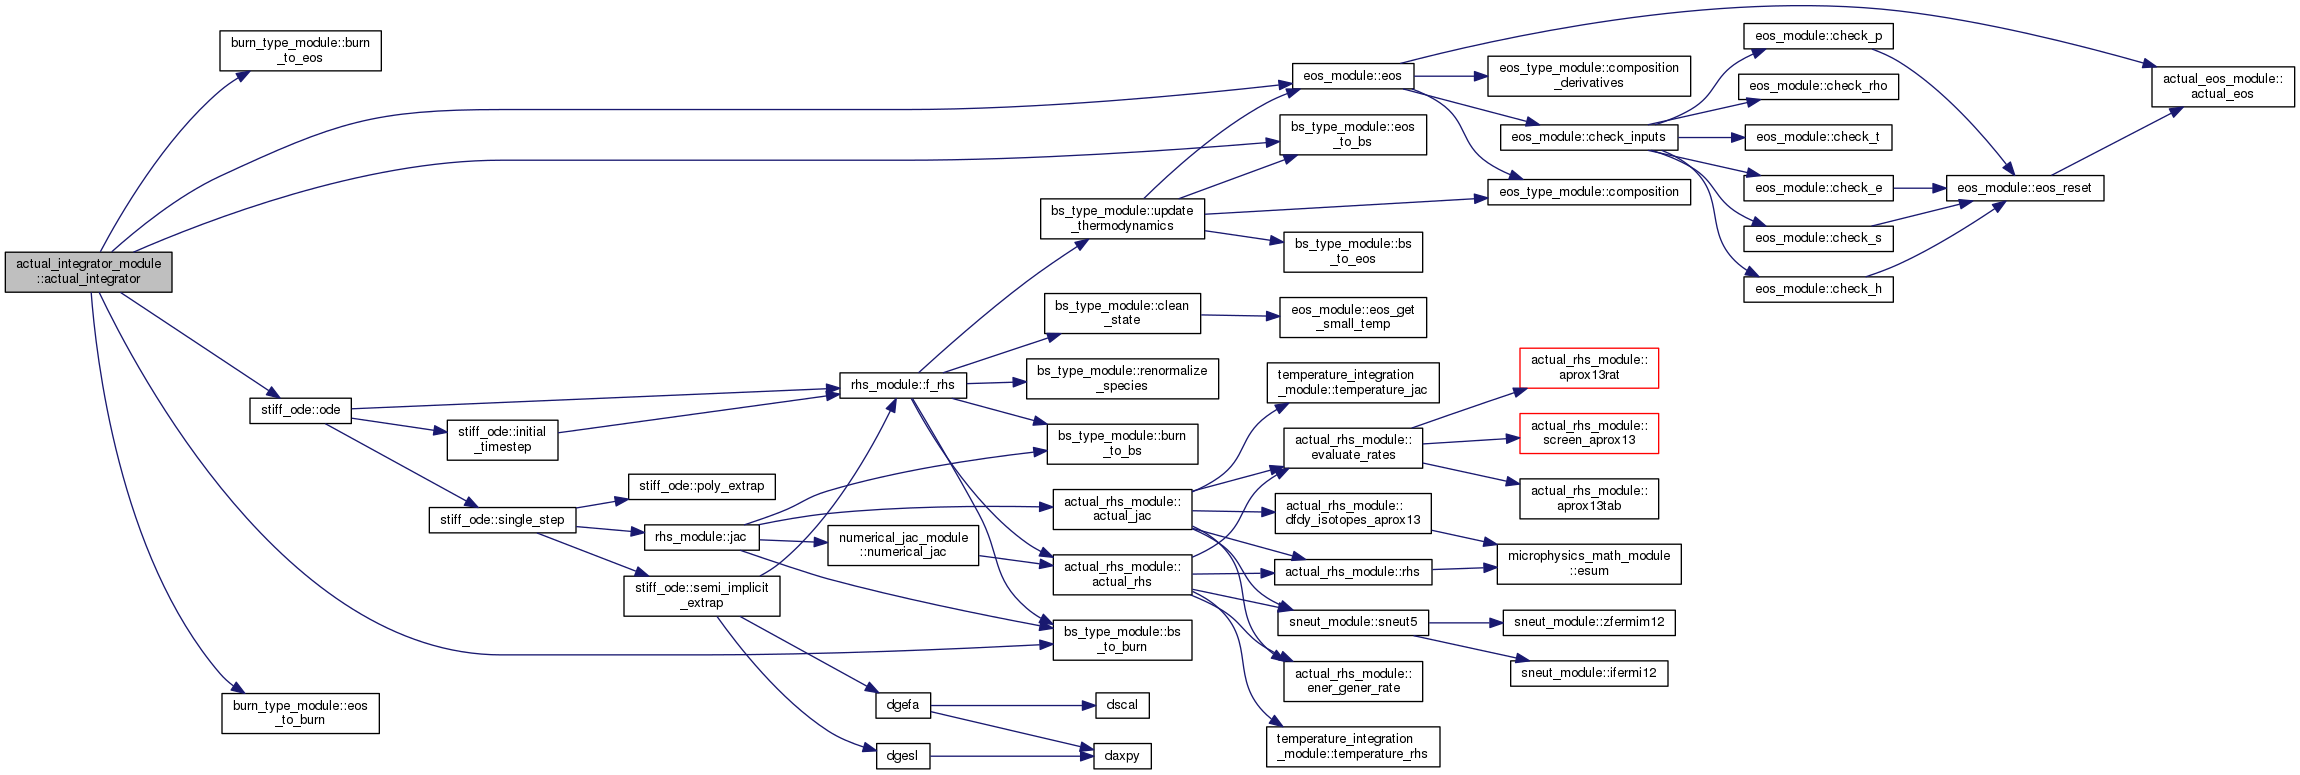
\includegraphics[width=\linewidth]{doxygen_network}
\end{sidewaysfigure}
